\documentclass[adobefonts, nocap]{ctexart}
\usepackage{amsmath}
\usepackage{amsfonts}
\usepackage{listings}
\usepackage{xcolor}
\usepackage{graphicx}
\usepackage{siunitx}
\usepackage{hyperref}
\hypersetup{
  colorlinks = true,
  linkcolor = blue,
  unicode = true
}
\lstset{
  language = C,
  basicstyle = \small\ttfamily,
  keywordstyle = \small\ttfamily\color{red},
  stringstyle = \color{gray},
  numbers = left,
  numberstyle = \tiny,
  numbersep = 5pt,
  frame = leftline,
  showstringspaces = false
}
\begin{document}
  \title{计算机系统结构第一次实验}
  \author{李雨田\hspace{1em}2010012193\hspace{1em}计14}
  \maketitle
  \tableofcontents
  \section{测量数据缓存的大小}
    \subsection{实验原理}
      测量数据缓存大小的基本思想是对一段大小的数组反复读取,并且逐次增加数组的大小.当数组的大小超过缓存的大小时,频繁读取就会导致频繁
      替换缓存,使得吞吐量下降.所以只要测量吞吐量,观察发生突变的点,即可得到缓存的大小.

      但是最新的Intel处理器自带硬件预读取功能,即会根据程序执行时读取内存的步长预测下一次访问,并且提前读取到缓存里.如果
      按照顺序访问数组的方法,则会发现吞吐量一直不会下降,或没有很明显的突变点,正是因为硬件预读取提前替换了缓存,没有影响到读取的效率.

      为了不让处理器预测出访问的步长,可以每次产生一个伪随机数作为下标访问.但是产生随机数本身就会影响程序计时,并且
      调用外部函数时会导致内存访问,使得之前的缓存失效.

      这里可以仿照链表的实现方式,把下一次访问的地址放在这次访问
      的地址所对应的变量中.每次读取内存的时候,把读到的值作为下一次访问的地址,防止硬件预读取工作.并且测量缓存大小时要适当增大步长,
      加大缓存替换的频率,使得结果更加明显.
    \subsection{实验结果和数据分析}
      运行程序,对$1$KB到$2048$KB之间大小的数组进行测试,并且得出吞吐量.吞吐量的单位是MB/s,但是因为使用\texttt{clock()}
      函数计时,结果并不是很准确.不过最重要的是吞吐量的相对大小,所以并不影响测量缓存的大小.

      程序源代码为\texttt{cache-size.c},运行时通过命令行提供两个参数,分别为起始和结束测量的大小.然后程序会给出相应大小
      下的吞吐量.

      程序输出如图\ref{fig1}所示,将结果画成折线图如图\ref{fig2}所示.注意到横轴对应的是$2^{x}$KB.
      从图中可以看出在$32$KB和$256$KB处有明显的吞吐量的突降,于是判断L1和L2数据缓存的大小分别为
      32KB和256KB.

      \begin{figure}[htbp]
        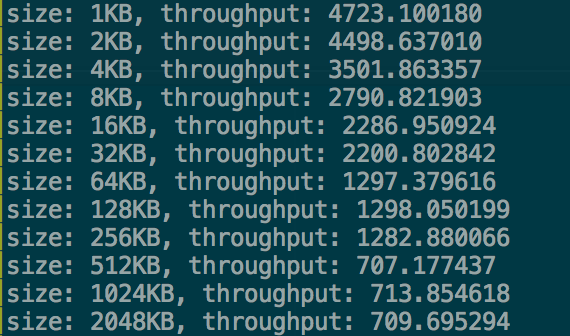
\includegraphics[width=12cm]{1.png}
        \caption{数据缓存大小程序输出}
        \label{fig1}
      \end{figure}

      \begin{figure}[htbp]
        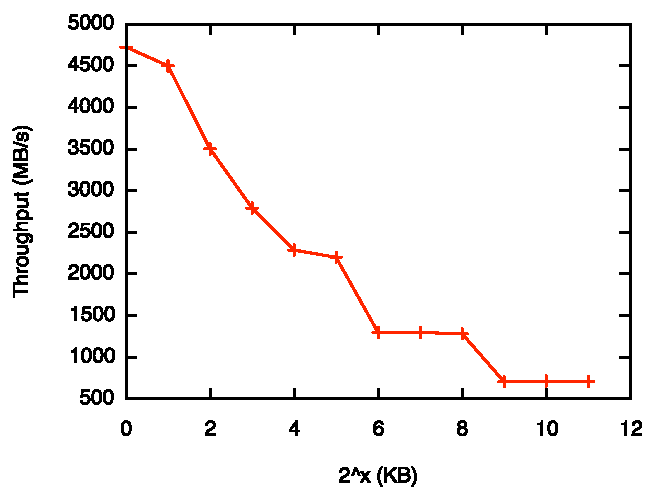
\includegraphics[width=12cm]{2.pdf}
        \caption{数据缓存大小数据}
        \label{fig2}
      \end{figure}
      \clearpage
  \section{测量数据缓存的块大小}
    \subsection{实验原理}
      同样是对内存进行顺序访问,但是只要读到块里的某一个字节,整个块都会被缓存进来.所以如果按顺序每字节均访问,那么仅仅会在访问该块的第一个
      字节的时候访问更低级存储.接下来在该块内的访问会直接命中.如果不是每个字节都依次访问,加大访问的步长,可以预见当步长等于块大小的时候,
      每一次读取就会要访问更低级存储,将整个块都加载进来,这样的吞吐量是最低的.

      所以采取每次加大步长的方法,观察吞吐量将会出现先降后升的现象,并且最低点对应的步长即正好是块大小.

      这里仍然要注意到硬件预读取带来的影响,同样使用类似链表的数据结构进行访问.
    \subsection{实验结果和数据分析}
      程序源代码为\texttt{block-size.c}.运行程序,对步长从$1$到$32$进行测试.这里的步长是指\texttt{uint64\_t}的长度,即$8$B.

      得到程序输出如图\ref{fig3},将结果画成折线图如图\ref{fig4}.程序前面在波动中下降,并当步长等于$8$,即$64$B的时候达到吞吐量的最低值.
      所以可以判断L1和L2数据缓存的块大小是$64$B.

      \begin{figure}[htbp]
        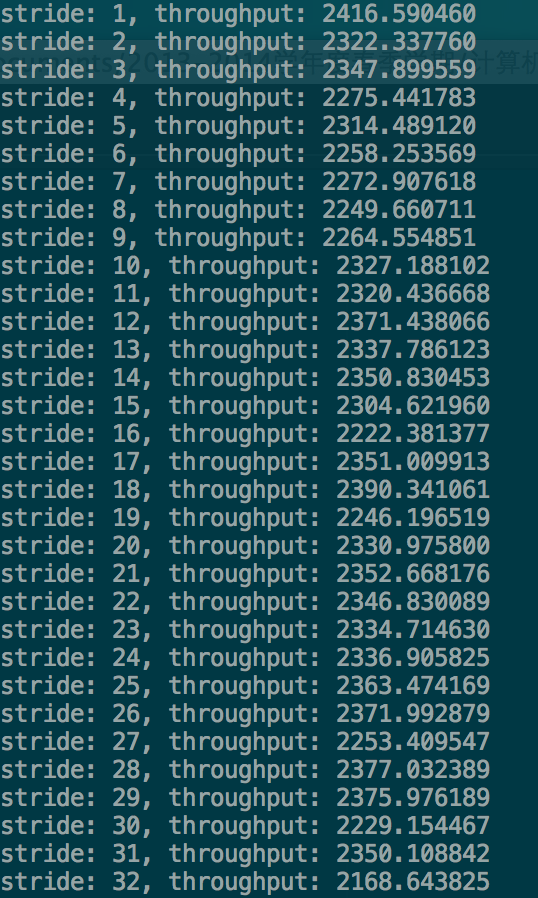
\includegraphics[width=12cm]{3.png}
        \caption{数据缓存块大小程序输出}
        \label{fig3}
      \end{figure}

      \begin{figure}[htbp]
        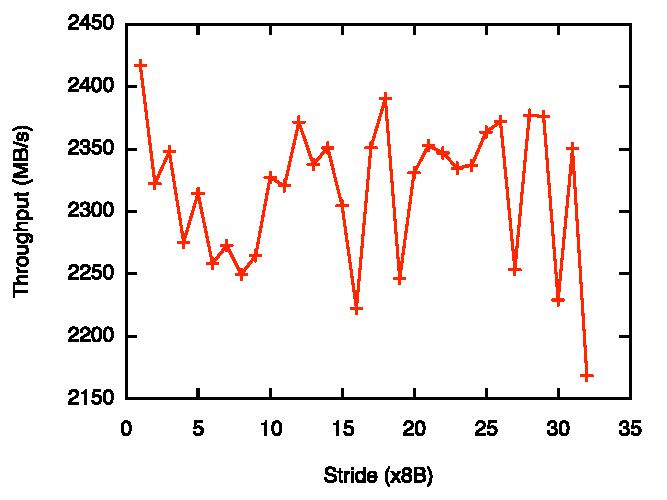
\includegraphics[width=12cm]{4.pdf}
        \caption{数据缓存块大小数据}
        \label{fig4}
      \end{figure}
      \clearpage
  \section{测量数据缓存的相连度}
    \subsection{实验原理}
      到现在已经知道块大小是$64$B,缓存的大小也已经测出来了.下面只要测出来一共有多少个组,就能知道每个组的大小和相连度了.

      已知块大小是$64$B,占了地址最低的$6$位.这里可以取一掩码,用来分割地址前面的标签和后面的索引和偏移量部分.实际上在程序实现时可以取这个掩码加$1$之后的值,
      每次往地址上累加.如果掩码没有盖住索引和偏移量部分,那么往地址上加的时候会改变索引,会从一个组跳到另一个组.如果掩码正好盖住
      或者超过了索引和偏移量,那么往地址上累加的时候就只会改变标签,而仍然还在同一个组内.

      所以通过枚举掩码长度,当掩码正好盖住索引和偏移量的时候,所有读取的内容都属于同一个缓存组,缓存冲突频率最大,吞吐量最低.通过观察
      吞吐量下降到极值的这个点,即可算出相连度.
    \subsection{实验结果和数据分析}
      程序源代码为\texttt{associativity.c}.依次左移掩码,得到程序输出如图\ref{fig5}.这里的\texttt{mask}实际上是掩码加$1$之后的值,
      即往地址上累加的值.

      数据如图\ref{fig6}.可以看出当掩码为$12$位的时候吞吐量最低,即可判断地址的低$12$位是索引和偏移量.已知偏移量为$6$位,所以索引为$6$位,共有$64$个不同的组.一级缓存共有$32$KB,而块大小之前已经算出来是64B,计算得到一组里有$8$个块,即是$8$相连的.

      考虑到一级缓存和二级缓存有一定的一致性,猜测二级缓存也是$8$相连的.之前已经得到二级缓存共$256$KB,算得一共应有$512$组.对应的掩码有$15$位,
      可以看到在图\ref{fig6}中当掩码为$15$位时,吞吐率的增长趋势得到抑制,验证猜测是正确的,即二级缓存也是$8$相连的.

      对于图\ref{fig6}后面吞吐量开始上升,是因为程序采用固定读取量,测量时间得到吞吐量的方法.当掩码变大时,实际上每一步跳跃距离变大,但数组大小不变,
      为了达到同样的读取量,只能多次重复读取.跳跃距离变大导致不同的地址的数量太少,可能会无法使缓存某一组填满,更不用说替换了,所以吞吐量
      会变高.要解决这个问题可以扩大数组的大小,但是实际上目前已经可以得到缓存的相连度,并没有这个必要.

      \begin{figure}[htbp]
        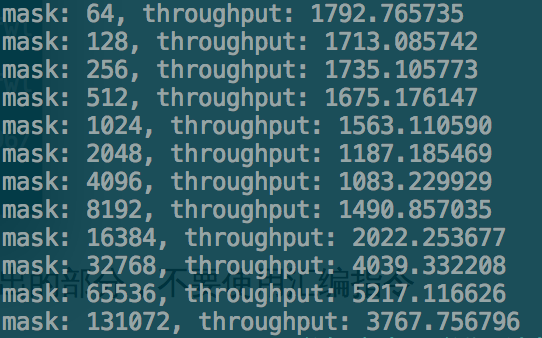
\includegraphics[width=12cm]{5.png}
        \caption{数据缓存相连度程序输出}
        \label{fig5}
      \end{figure}

      \begin{figure}[htbp]
        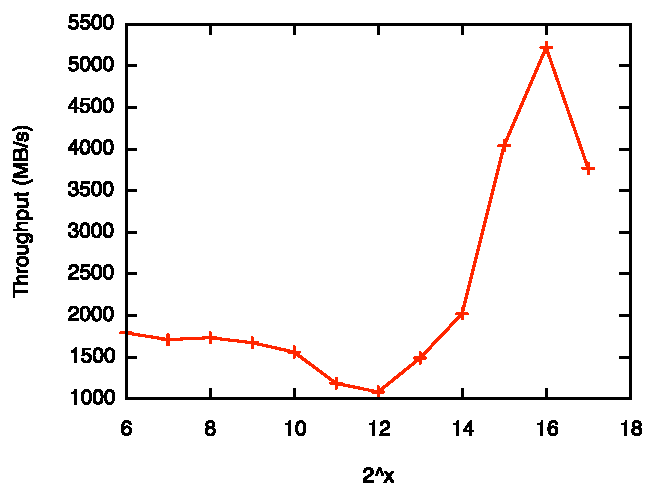
\includegraphics[width=12cm]{6.pdf}
        \caption{数据缓存相连度数据}
        \label{fig6}
      \end{figure}
      \clearpage
  \section{对所给程序\texttt{matrix\_mul.cpp}进行优化}
    对于$A\times B=C$的矩阵乘法.对于指数的顺序,一共有三种方式.其中$ijk$和$jik$等效, $jki$和$kji$等效, $kij$和$ikj$等效.

    根据\textit{Computer Systems A Programmer's Perspective}上的结论,有如表\ref{tab1}所示结论.

    所以只要采用$kij$或者$ikj$方式,就能大幅利用空间局部性提高效率.

    改进后程序输出如图\ref{fig9}所示.经测试使用原来的方法耗时\SI{8292664}{\ms},使用$ikj$方式只需\SI{2781312}{\ms},时间减少
    $66.46\%$.

    为了进一步提高程序的运行效率,可以采用矩阵分块的思想,增大空间局部性.$A$为$1000\times 1000$的矩阵,每个元素占$4$B,一行为$4000$B.
    考虑到一级缓存为$32$KB,分到$A$, $B$, $C$三个矩阵上,每个矩阵大概可以利用$10$KB.所以在$ikj$的方式上进一步改进,每次对$i$, $i+1$, $i+2$,
    $i+3$同时操作,降低$B$的重复读取的次数.这时的程序源代码为\texttt{matrix\_mul.cpp},程序输出如图\ref{fig10}所示,时间减少$71.77\%$.

    如果还想进一步优化,可以使用编译器的优化参数\texttt{-O3},得到程序输出如图\ref{fig11}所示,时间减少达到$95.98\%$,性能提升巨大.可能因为
    循环次数是常数,编译器直接进行循环展开,再加上其它一些优化,才能得到这样的结果.

    \begin{table}[htbp]
      \caption{矩阵乘法效率}
      \label{tab1}
      \centering
      \begin{tabular}{p{1.5cm} p{1.5cm} p{1.5cm} p{1.5cm} p{1.5cm} p{1.5cm} p{1.5cm}}
        Matrix multiply version & Loads per iter. & Stores per iter. & A misses per iter. & B misses per iter. & C misses per iter. & Total misses per iter. \\
        \hline
        $ijk$ \& $jik$ & 2 & 0 & 0.25 & 1.00 & 0.00 & 1.25 \\
        $jki$ \& $kji$ & 2 & 1 & 1.00 & 0.00 & 1.00 & 2.00 \\
        $kij$ \& $ikj$ & 2 & 1 & 0.00 & 0.25 & 0.25 & 0.50 \\
      \end{tabular}
    \end{table}

    \begin{figure}[htbp]
      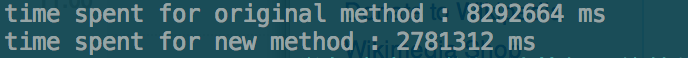
\includegraphics[width=12cm]{9.png}
      \caption{优化矩阵乘法程序输出一}
      \label{fig9}
    \end{figure}

    \begin{figure}[htbp]
      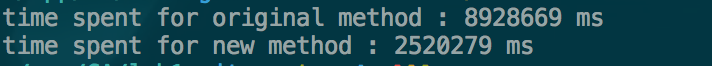
\includegraphics[width=12cm]{10.png}
      \caption{优化矩阵乘法程序输出二}
      \label{fig10}
    \end{figure}

    \begin{figure}[htbp]
      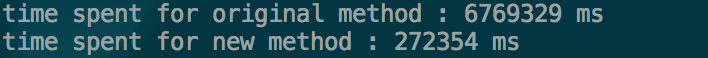
\includegraphics[width=12cm]{11.png}
      \caption{优化矩阵乘法程序输出三}
      \label{fig11}
    \end{figure}
    \clearpage
  \section{测量数据缓存的写策略}
    \subsection{实验原理}
      数组大小小于缓存大小时,如果是采用的写回法,则没有对低级存储的访问,而如果是采用的写直达法,则每次都会访问低级存储.但是当数组大小大于缓存大小时,无论采用哪种方法,都会对低级存储进行写操作.于是可以通过比较这两种情况下的吞吐量的差别,来测量数据缓存的写策略.

      为了增大可能存在的性能上的差别,每次访问的步长正好是一个块大小.这样就能在最短时间内写脏整个数据缓存,扩大吞吐量的差距.
    \subsection{实验结果和数据分析}
      程序源代码为\texttt{write-back.c}.运行得到程序输出如图\ref{fig7}.当数组大小正好为一级缓存大小时,吞吐量有$1872.55$MB/s,而当数组大小超过
      一级缓存大小时,吞吐量下降到$1790.69$MB/s,下降了$4.4\%$.多次测量均可观测到这个差距,说明数据缓存采用写回法.

      \begin{figure}[htbp]
        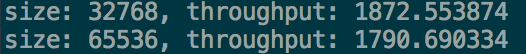
\includegraphics[width=12cm]{7.png}
        \caption{数据缓存写策略程序输出}
        \label{fig7}
      \end{figure}
  \section{测量数据缓存的替换策略}
    \subsection{实验原理}
      此时已经知道缓存的基本大小信息,可以通过巧妙地构造访问序列,来测试缓存的替换策略.这里构造两个序列,其中一个对FIFO有特别优化,另一个对LRU有特别优化,但是两者的总
      访问量保持相当.这样如果一个序列访问时间短,另一个访问时间长,就可以以此来判断数据缓存的替换策略.

      一个缓存组里面有$8$个块,所以一共需要$9$个块,编号为$0$到$8$.注意到它们的地址的后$12$位是相同的,即都属于同一个组.构造出对FIFO有特别优化的序列是\texttt{081102213324435546657768870},对LRU有特别优化的序列是\texttt{080212434656878101323545767}.可以看出FIFO序列中有$n,n-1,n+1$类型元素,
      如果采用LRU会打乱$n$和$n+1$的顺序,使得缓存替换增多.同样LRU序列中有$n,n-1,n$类型元素,如果采用FIFO则会使得第二次访问$n$的时候发生缓存替换.

      最后需要注意在执行完一个序列之后缓存要恢复成原样,这里设为\texttt{01234567}.只有这样才能反复测量,得到比较明显的结果.
    \subsection{实验结果和数据分析}
      程序源代码为\texttt{replacement.c}.运行程序输出如图\ref{fig8}.看出运行LRU序列的时间比FIFO的少$11.55\%$,得到缓存采用的替换策略是LRU.

      实际上通过搜索知道,此CPU的缓存采用的是LRU的变种PLRU.并不是严格地按照最近访问先后顺序替换缓存,但是大致上是和最近访问相关,最近访问越久远的缓存更有可能被替换出去,
      符合测量结果的判断.

      \begin{figure}[htbp]
        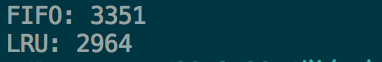
\includegraphics[width=12cm]{8.png}
        \caption{数据缓存替换策略程序输出}
        \label{fig8}
      \end{figure}
\end{document}
